\subsection{Sytuacje obsługiwane przez system}

Tworzony system będzie w stanie obsługiwać następujące sytuacje:

\begin{itemize}
	\item Rysowanie pomocniczych linii poziomych
	\begin{itemize}
		\item Na obrazie z kamery rysowane są statyczne linie pomocnicze mające na celu wspomaganie kierowcy przy parkowaniu
		
		\begin{center}
			Zdjęcie poniżej przedstawia przykładową wizualizacje linii pomocniczych
		\end{center}
		
		\begin{figure}[H]
			\centering
			\resizebox{\columnwidth}{!}{
				\includegraphics{Img/linie_pomocnicze.png}
			}
			\caption{Linie pomocnicze są nakładane na obraz z kamery}
			\label{fig:linie}
		\end{figure}
	\end{itemize}
	\newpage
	\item Wykrywanie pieszych znajdujących się przed lub za samochodem
	\begin{itemize}
		\item Po wykryciu pieszego w polu widzenia kamery system informuje o tym kierowcę w wybrany w konfiguratorze sposób. \newline
		\begin{center}
			Zdjęcie poniżej pokazuje przykład tego typu sytuacji:
		\end{center}

		\begin{figure}[H]
			\centering
	 		\resizebox{\columnwidth}{!}{
				\includegraphics{Img/pieszy.png}
			}
       		\caption{Wykryty pieszy zostaje oznaczony przez system}
			\label{fig:pieszy}
		\end{figure}
	\end{itemize}
	
	\newpage
	
	\item Wykrywanie znaku Stop oraz znaków z grupy znaków ostrzegawczych
	\begin{itemize}
		\item Kiedy w polu widzenia kamery zostanie wykryty jeden z rozpoznawanych znaków kierowca zostanie o tym poinformowany w wybrany w konfiguratorze sposób.
		
		\begin{center}
			Zdjęcie poniżej pokazuje przykład tego typu sytuacji:
		\end{center}
		
		\begin{figure}[H]
			\centering
			\resizebox{\columnwidth}{!}{
				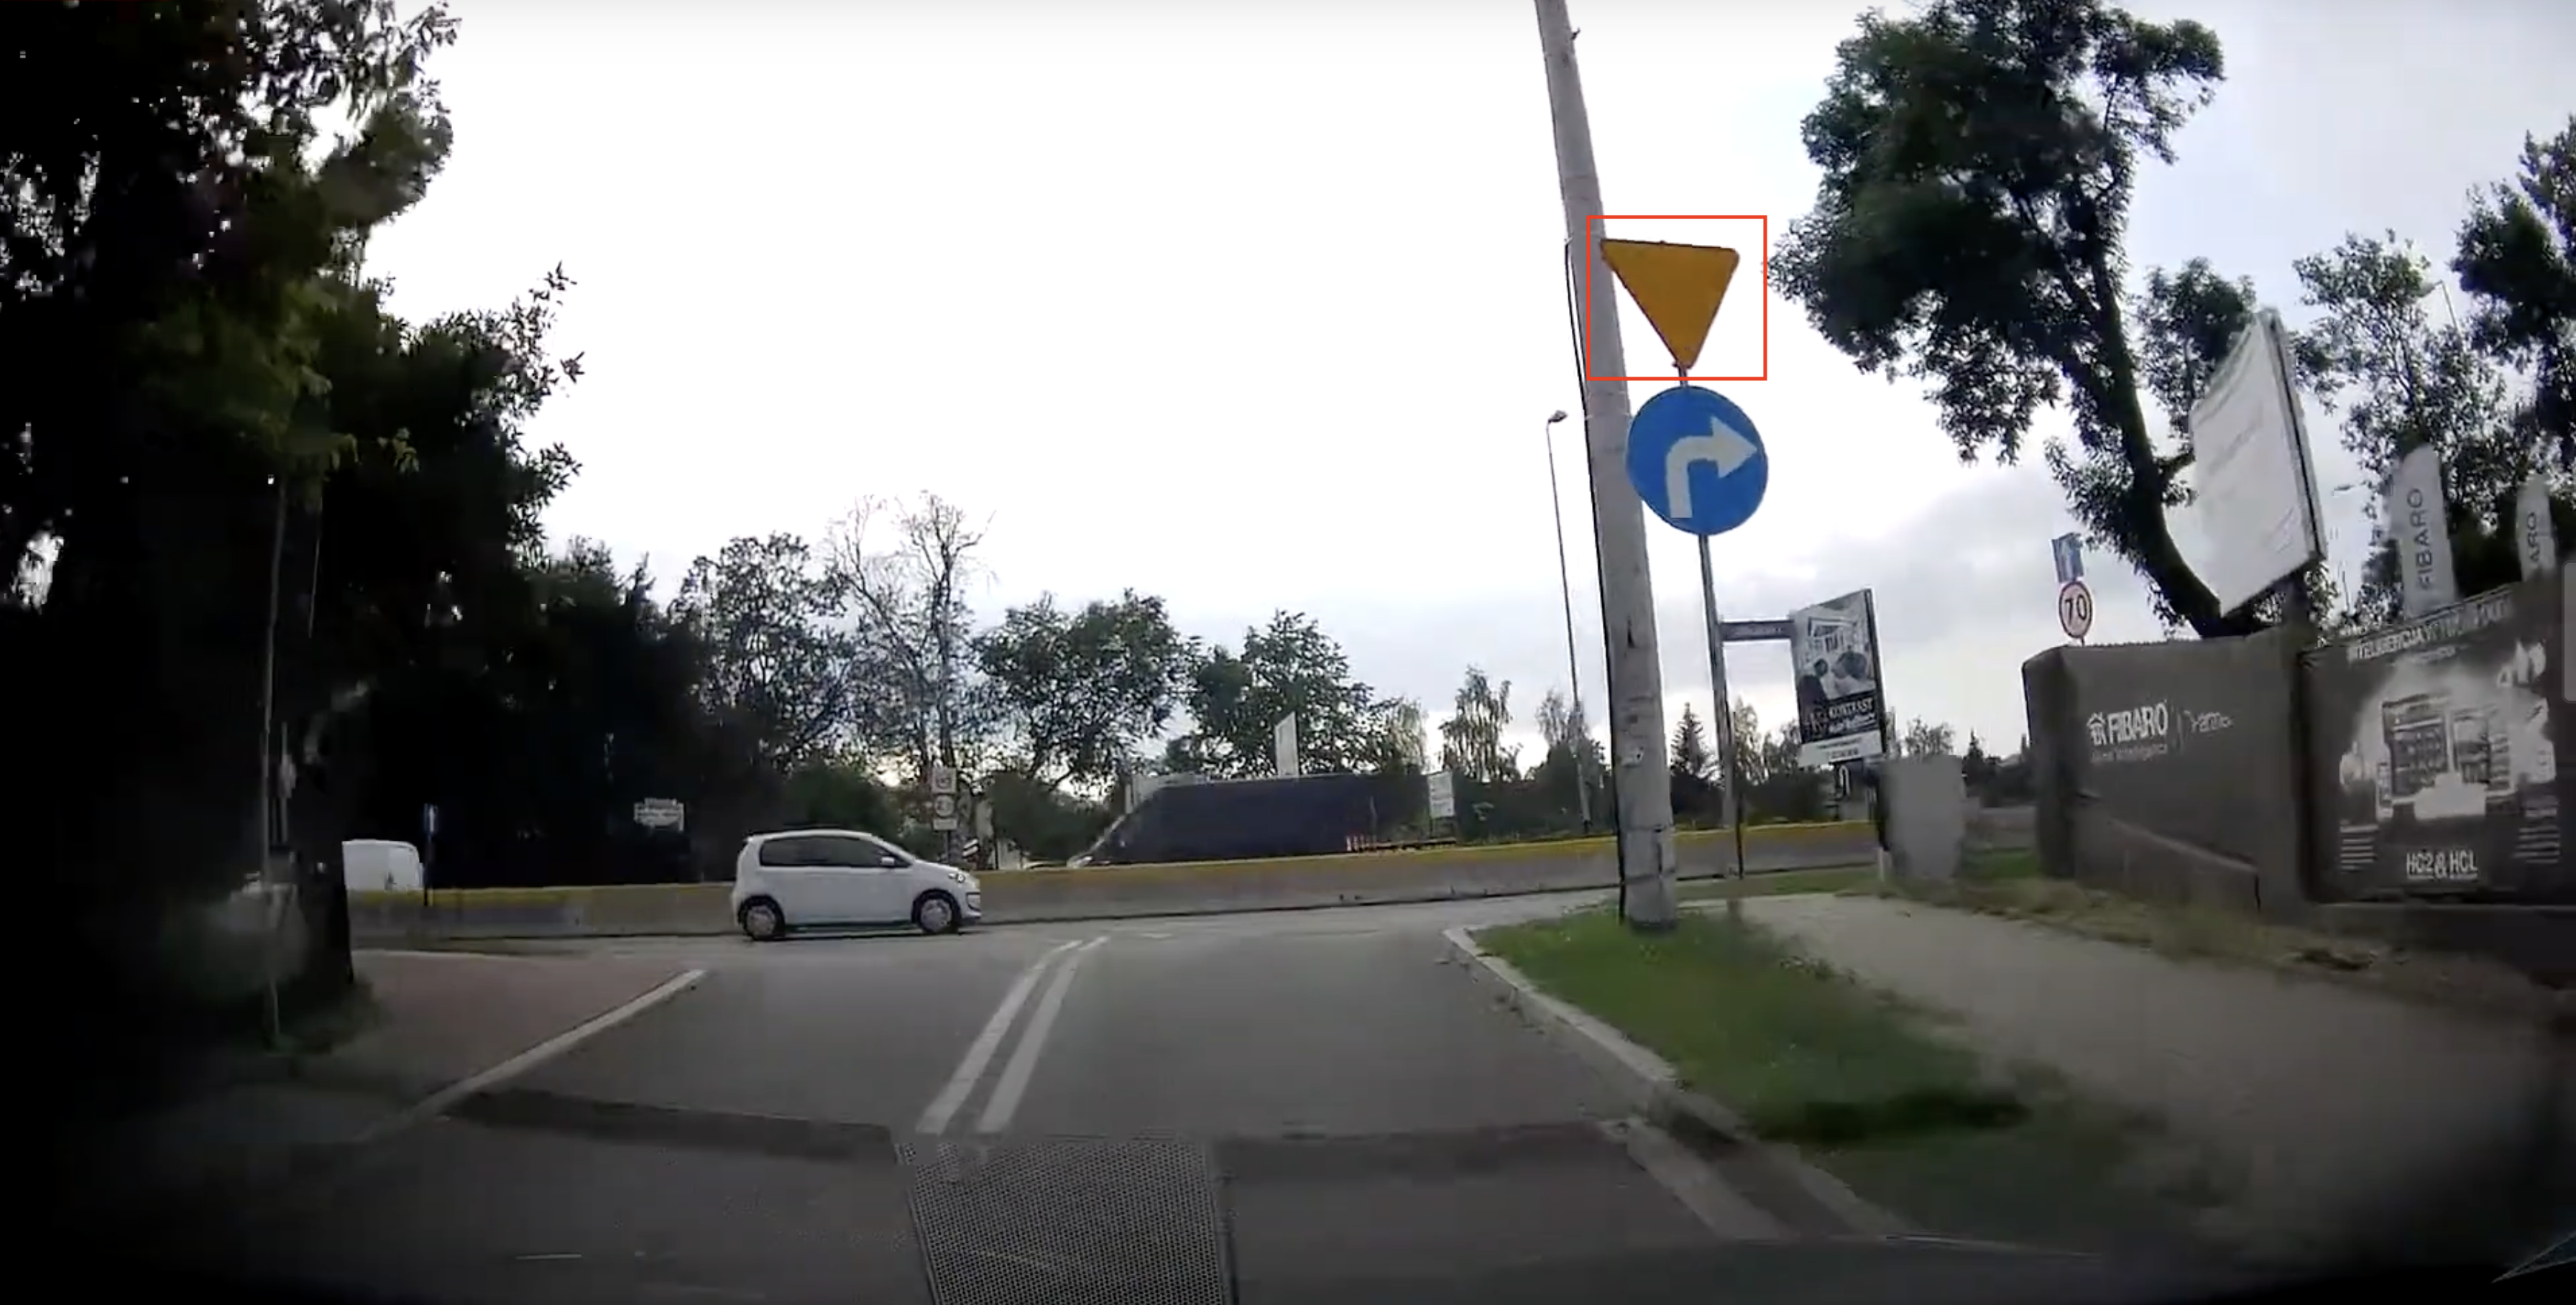
\includegraphics{Img/znak_ostrzegawczy.png}
			}
			\caption{Wykryty znak ostrzegawczy zostaje oznaczony przez system}
			\label{fig:znak}
		\end{figure}
		
	\end{itemize}
	
	\newpage
	
	\item Wykrywanie innych samochodów
	\begin{itemize}
		\item Kiedy system wykryje samochód w polu widzenia kamery, poinformuje on o tym kierowcę, w sposób wybrany w konfiguratorze.
		
		\begin{center}
			Zdjęcie poniżej pokazuje przykład tego typu sytuacji:
		\end{center}
		
		\begin{figure}[H]
			\centering
			\resizebox{\columnwidth}{!}{
				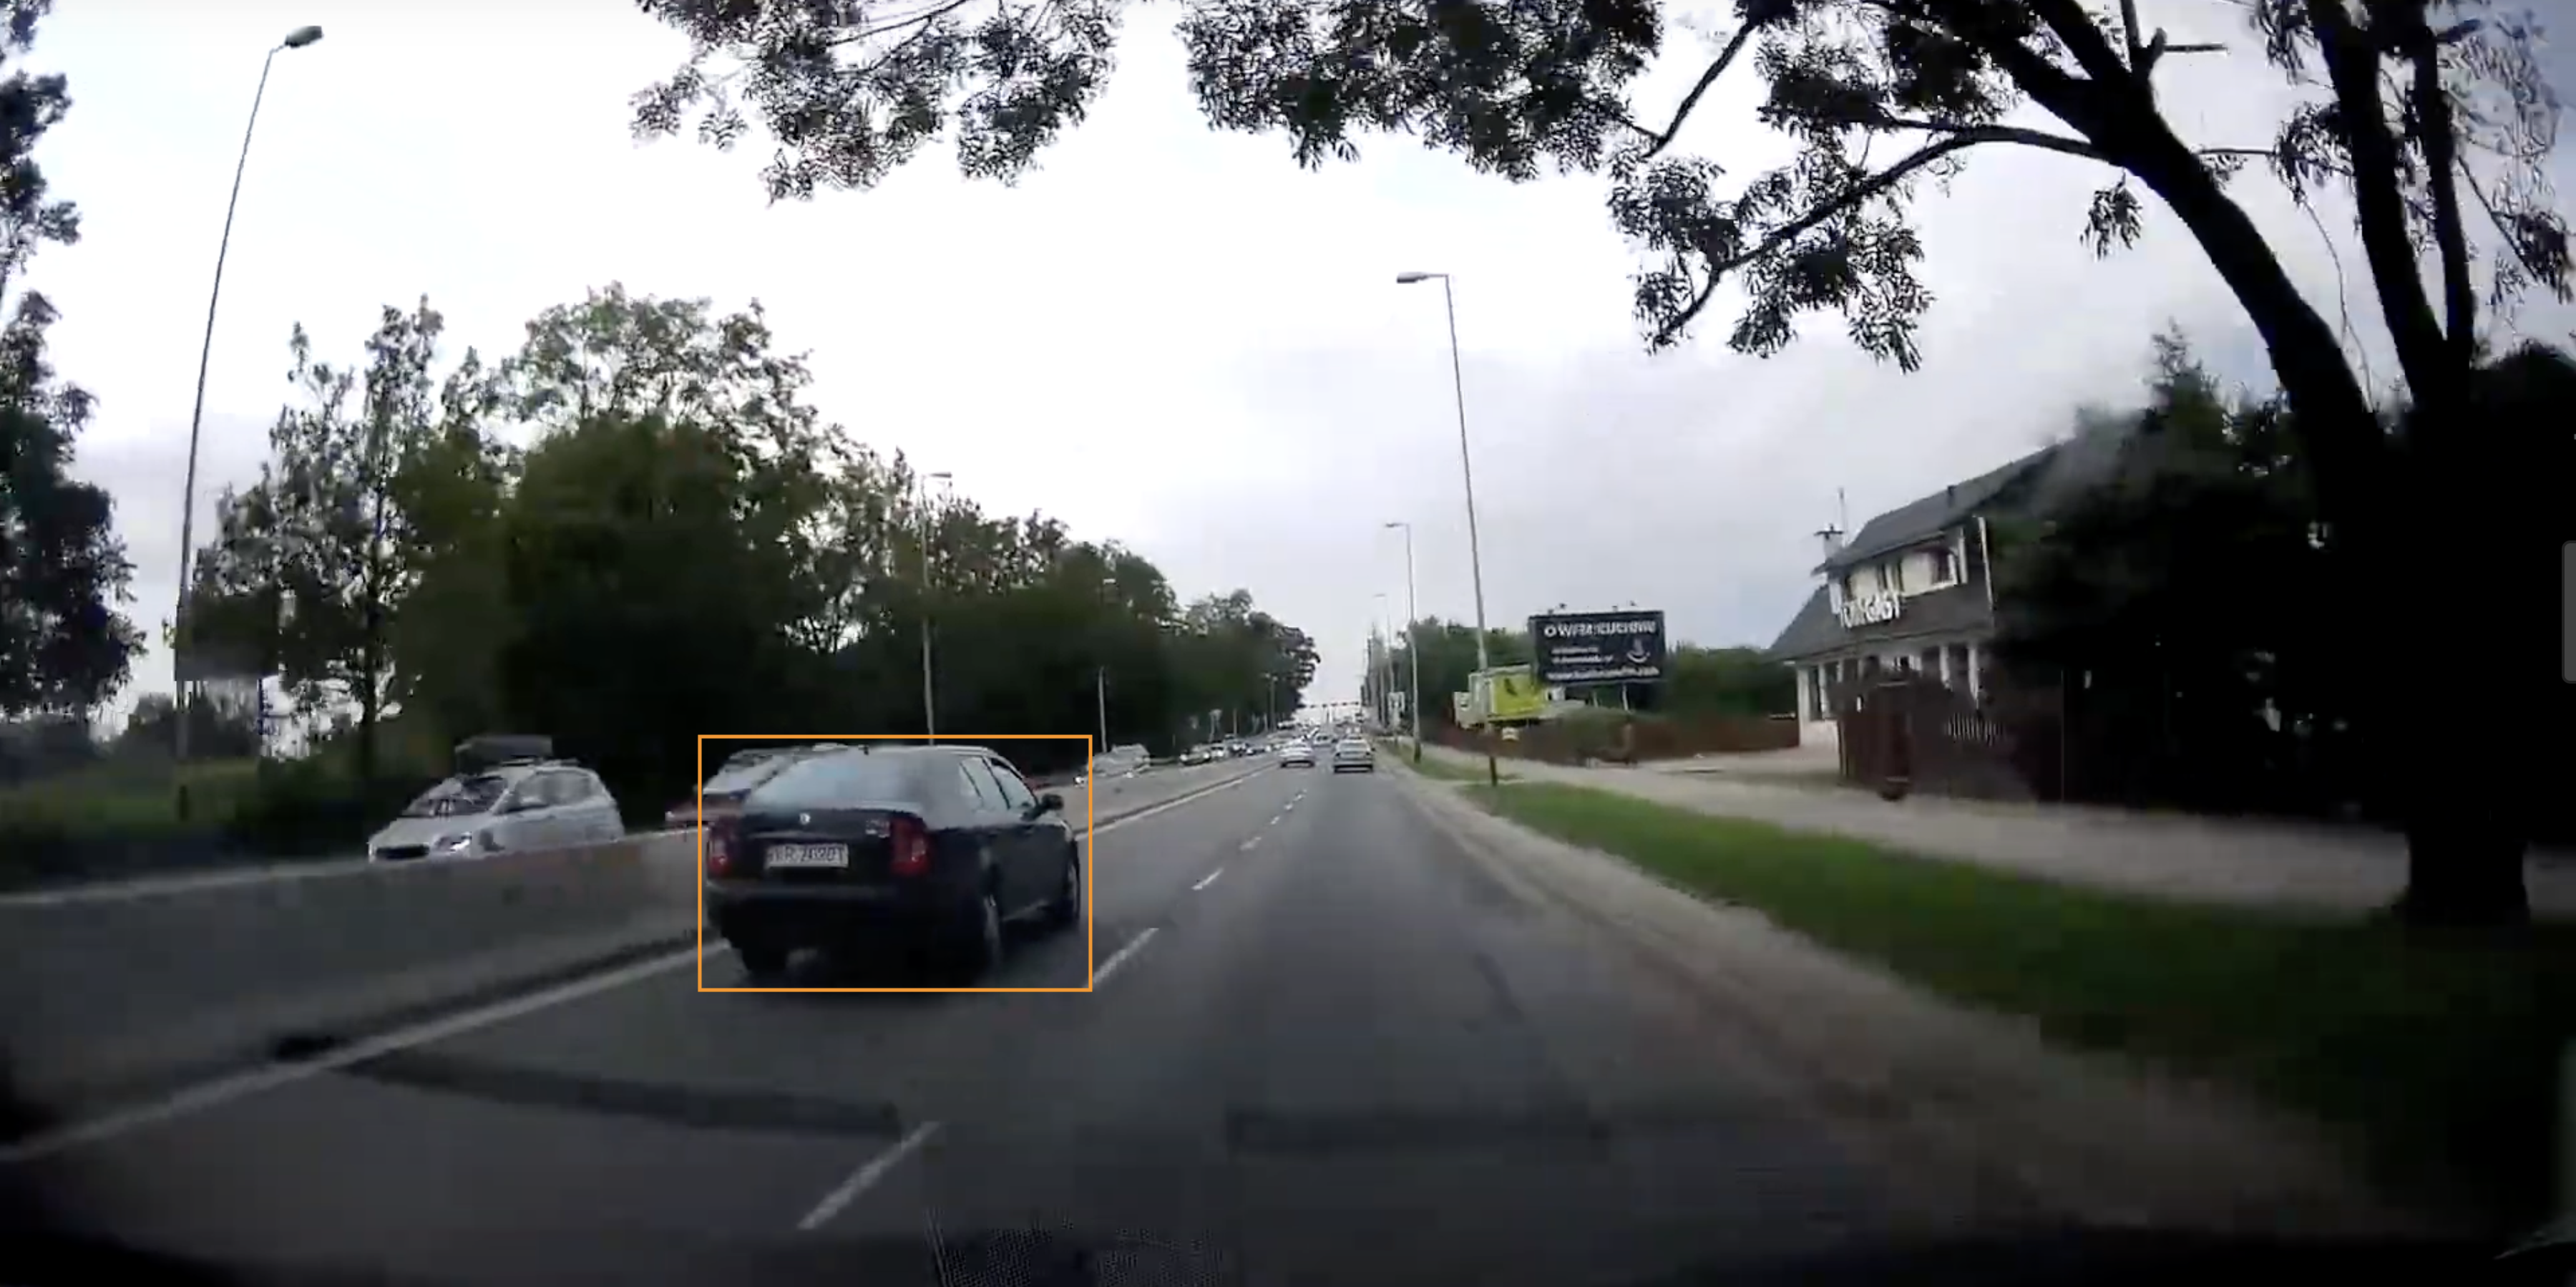
\includegraphics{Img/inny_samochod.png}
			}
			\caption{Wykryty samochód zostaje oznaczony przez system}
			\label{fig:samochod}
		\end{figure}
		
	\end{itemize}
\end{itemize}
  

  
